%Farid
\chapter{Comparaison avec un Asservissement avec Correction Proportionnelle  et Retour Tachymétrique }
\chaptermark{Comparaison} 
\subsection{Retour de sortie avec correcteur proportionnelle}

on considère l'asservissement de position:\\
\begin{center}
$V_m(t)=k_1'(V_r(t)-V_s(t))=k_1'K_e(\theta_r(t)-\frac{K_s}{K_e}\theta_s(t)$
\end{center}
Avec $k_1'$>0 et ici,$K_e=K_s$. il représenter  ci-dessous:
\\


\begin{center}
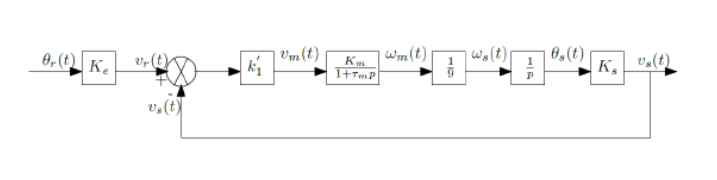
\includegraphics[scale=0.5]{fiiig3.png} 
\captionof{figure}{\textit Asservissement de position avec correction proportionnelle}
\label{fig3}
\end{center}


\subsubsection{Représentation d'état de l'asservissement}
$\omega$=$X_2 et V_s=X_1$

\begin{equation*}
\left\{\begin{matrix}
\dot{x}(t)=Ax(t)+Bu(t)\\ 
y(t)=Cx(t)+Du(t)\\
\end{matrix}\right.
\end{equation*}   


$X_1$=$\frac{K_S}{9p}X_2$\\\\


$X_2$=$\frac{K_mk_1'}{1+Tmp}(V_r-X_1)$\\

\begin{equation*}
\begin{matrix}
\dot{X_1}=\frac{K_s}{9}X_2\\
\dot{X_2}=-\frac{X_2}{T_m}-\frac{K_mk_1'}{T_m}-\frac{K_mk_1'}{Tm}V_r
\end{matrix}
\end{equation*}
\\

L'equation d'etat est:\\\\


$\dot{X}$=$\begin{bmatrix}
0&\frac{K_s}{9}\\
-\frac{K_mk_1'}{T_m}&-\frac{1}{T_m}
\end{bmatrix}X
\quad + \quad
\begin{bmatrix}
0\\
\frac{K_mk_1'}{T_m}
\end{bmatrix}V_r
$

\subsection{Expression de la fonction de transfert}


\begin{center}
$H(p)=\frac{1}{\frac{9T_m}{K_sk_1'K_m}}p^2+\frac{9}{K_sk_1'K_m}p+1$
\end{center}


Le gain statique est 1.
La pulsation naturelle $\omega_n=\sqrt{\frac{K_sk_1'K_m}{9T_m}}$
%L'amortissement $\zeta=\frac{3}{2\sqrt{(T_mK_sK_mk_1')}}$

\subsubsection{Erreur de position $\epsilon_p$}
$\epsilon_p=\lim\limits_{\substack{p \rightarrow 0 }} 1-H(p)$\\
$\epsilon_p=0$

\subsubsection{Erreur de trainage à une rampe $\epsilon_r$}
$\epsilon_r=\lim\limits_{\substack{p \rightarrow 0 }} \frac{1-H(p)}{p}$
$\epsilon_r=2$

Avec la commande MATLAB "rlocus" ce qui nous as permet de  tracer le lieu sur lequel peut  positionner les pôles de l'asservissement voir la figure.



\begin{center}
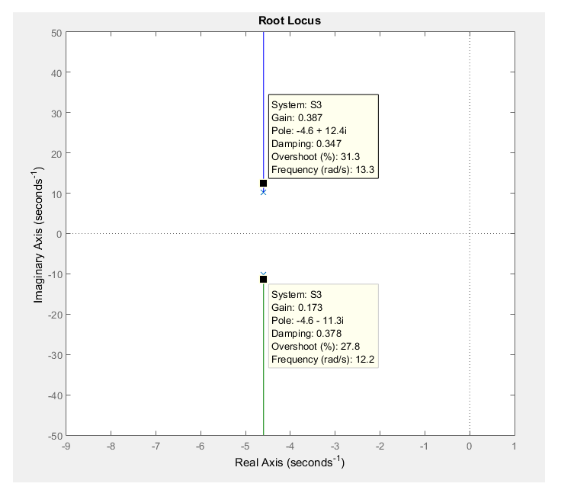
\includegraphics[scale=0.5]{fiiig4.png}
\captionof{figure}{\textit Lieu des pôles de l'asservissement}
\label{fig4} 
\end{center}

\subsection{Mise en place d'une contre réaction tachymétrique}


\begin{center}
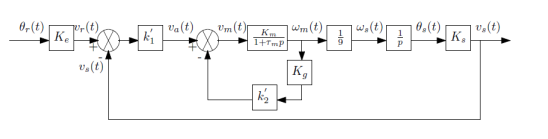
\includegraphics[scale=0.5]{fiiig5.png} 
\captionof{figure}{\textit Asservissement de position avec contre-réaction tachymétrique}
\end{center}
On met un correcteur tachymétrique dans le schéma précédent.

\subsection{Fonction de transfert de la boucle interne de vitesse}

$\omega_m=\frac{(\frac{K_m}{1+K_gk_1'K_m})}{1+(\frac{T_m}{1+K_gk_1'K_m})p}$

$\Rightarrow K_0$=$\frac{K_m}{1+K_gk_2'K_m}$ 
 $\tau$=$\frac{T_m}{1+K_gk_2'K_m}$


%
%$\omega_m=\frac{(\frac{K_m}{1+K_gk_1'K_m})}{1+(\frac{T_m}{1+K_gk_1'K_m})p}$
%\\
%
%\Rightarrow $K_0=\frac{K_m}{1+K_gk_2'K_m}$ et $\tau=\frac{T_m}{1+K_gk_2'K_m}$